\documentclass[11pt]{beamer}
\usepackage{verbatim}
\usepackage{amsmath}
\usepackage{amsthm}
\usepackage{graphics}
\usepackage{color}
\usepackage{stmaryrd}\usefonttheme[onlymath]{serif}

\title{Discussion}
\date{\today}

\begin{document}
\maketitle
\begin{frame}\frametitle{Limitation of Nested Ranking Functions}

\begin{example}

\[\texttt{while }(x > 0 \vee y > 0) \]
\[\{\texttt{if }(y > 0): y' = y - 1; x ' = x;\texttt{else }: x' = x - 1;\}\]
\end{example}

\end{frame}


\begin{frame}\frametitle{Blocks}
Idea: use terms of the loop guard to split the space into \textit{blocks}.
\begin{center}

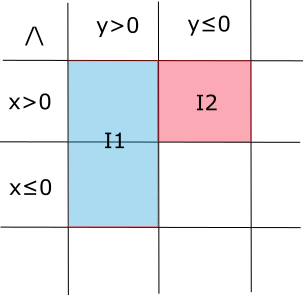
\includegraphics[scale = 0.65]{block.png}

\end{center}
\end{frame}
\begin{frame}\frametitle{Cyclic Dependency and Irregular Split}

\begin{example}

\[\texttt{while }(x > 0 \vee y > 0) \]
\[\{\texttt{if }(y > 0): y' = y - 2; x ' = x;\texttt{else }: y' = y + 1;x' = x - 1;\}\]

Start with $x = 1, y = 5$


A possible single linear ranking function $f(x, y) = x + 3y$.

This example demonstrates the blocks may be split by the ranking function. 

i.e. in last example the regular split is just a coincidency.

\end{example}

\end{frame}

\begin{frame}\frametitle{Blocks}
Use the terms of a loop 
\begin{center}

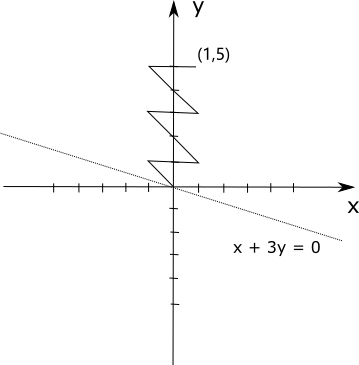
\includegraphics[scale = 0.65]{jump.png}

\end{center}
\end{frame}

\begin{frame}\frametitle{Multiphase Cyclic Dependency}
\begin{example}

\[\texttt{while }(x > 0 \vee y > 0) \]
\[\{\texttt{if }(y > 0): x' = x - 2z; y' = y; z' = z + 1;\]
\[\texttt{else }: x' = x + z; y' = y - 1; z' = z;\}\]
\end{example}

Start from $x = 1, y = 8, z = -2$.



\end{frame}



\begin{frame}\frametitle{Guess $f_1$ for Multiphase Ranking Function}
Idea: although some ranking functions are not the borders of the blocks, we still wish to use the guard to guess the phases.

After a guess, conjunct the negation of the guard into the loop for nest guess.

The examble below shows that this idea is not feasible.
\begin{example}

\[\texttt{while }(x > 0 \vee y > 0) \]
\[\{\texttt{if }(y > 0): y' = y - 1; x' = 5;\]
\[\texttt{else }: x' = x - 1; y = 5; \}\]

\end{example}
The loop is not terminating but...
\end{frame}

\begin{frame}\frametitle{Attempt to Merge the Blocks}
Idea: if we find the jump-in-and-out situations of the execution between two blocks, we consider it as one.

Problem: One cannot tell it is the problem of the inability of multiphase ranking function for this loop, or it is really that these two blocks should be merged.

\end{frame}


\end{document}